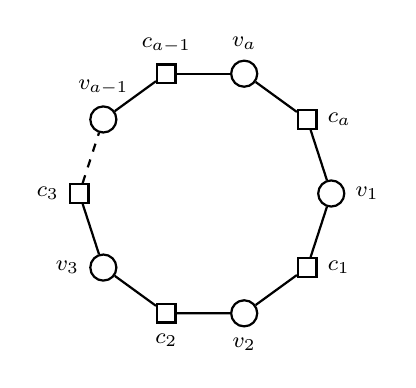
\begin{tikzpicture}[thick,scale=0.8]

% Draw the nodes in polar coordinates

%%%%%%%%%%%%%%%%%%%% Outer Cycle %%%%%%%%%%%%%%%%%%%%%%%%%%

%variable nodes
\foreach \index in {1}
{
    \node[circle, draw=black, label={right: \footnotesize{$v_{\index}$}}] (v1) at ({-((\index-1)*72)}:2) {};
}

\foreach \index in {2}
{
    \node[circle, draw=black, label={below: \footnotesize{$v_{\index}$}}] (v2) at ({-((\index-1)*72)}:2) {};
}

\foreach \index in {3}
{
    \node[circle, draw=black, label={left: \footnotesize{$v_{\index}$}}] (v3) at ({-((\index-1)*72)}:2) {};
}


\node[circle, draw=black, label={above: \footnotesize{$v_{a-1}$}}] (v4) at ({-((4-1)*72)}:2) {};

\node[circle, draw=black, label={above: \footnotesize{$v_{a}$}}] (v5) at ({-((5-1)*72)}:2) {};


%check nodes
\foreach \index in {1}
{
    \node[shape=rectangle, draw=black, label={right: \footnotesize{$c_{\index}$}}] (c\index) at ({-((\index-1)*72+36)}:2) {};
}

\foreach \index in {2}
{
    \node[shape=rectangle, draw=black, label={below: \footnotesize{$c_{\index}$}}] (c\index) at ({-((\index-1)*72+36)}:2) {};
}

\foreach \index in {3}
{
    \node[shape=rectangle, draw=black, label={left: \footnotesize{$c_{\index}$}}] (c\index) at ({-((\index-1)*72+36)}:2) {};
}

\node[shape=rectangle, draw=black, label={above: \footnotesize{$c_{a-1}$}}] (c4) at ({-((4-1)*72+36)}:2) {};

% \node[shape=rectangle, draw=black, label={[label distance=-0.55cm,auto,swap, font=\footnotesize] $c_{a}$}] (c5) at ({-((5-1)*72+36)}:2) {};

\node[shape=rectangle, draw=black, label={right: \footnotesize{$c_{a}$}}] (c5) at ({-((5-1)*72+36)}:2) {};


%Draw outer cycle
\foreach \index in {1, ...,2,3}
{
    \path [-,thick] (v\index) edge node[left] {} (c\index);  
}
\foreach \index in {1, 2}
{
    \path [-,thick] (c\index) edge node[left] {} (v\the\numexpr\index+1\relax);  
}

\foreach \index in {4,5}
{
    \path [-,thick] (v\index) edge node[left] {} (c\index);  
}
\foreach \index in {4}
{
    \path [-,thick] (c\index) edge node[left] {} (v\the\numexpr\index+1\relax);  
}

\foreach \index in {3}
{
    \path [dashed,thick] (c\index) edge node[left] {} (v\the\numexpr\index+1\relax);  
}

\path [-,thick] (c5) edge node[left] {} (v1);  

\end{tikzpicture}



